% no notes
%\documentclass{beamer}
% notes and slides
\documentclass[notes]{beamer}
% notes only
%\documentclass[notes=only]{beamer}
\usepackage{graphicx} % Allows including images
\usepackage{booktabs} % Allows the use of \toprule, \midrule and \bottomrule in tables
\usepackage{multirow}
\usepackage{multimedia}
\usepackage{tikz}
\usepackage{circuitikz}
\usepackage{url}
\usepackage{pgfplots}
\pgfplotsset{compat=newest}
\usepgfplotslibrary{groupplots,dateplot}
\usetikzlibrary{patterns,shapes.arrows}
\usepackage{standalone}
\usepackage{adjustbox}
\usepackage{lmodern}
\usepackage{pgfplots}
\usepackage{amsmath}
\usepackage{amsthm}
\usepackage{multimedia}
\usepackage{standalone}
\usepackage{csquotes}
\usepackage{hyperref} %links
\usepackage{url}
\usepackage{csquotes}

\PassOptionsToPackage{american}{babel} % change this to your language(s), main language last
% Spanish languages need extra options in order to work with this template
% \PassOptionsToPackage{spanish,es-lcroman}{babel}
\usepackage{babel}

\PassOptionsToPackage{%
  backend=biber,bibencoding=utf8, %instead of bibtex
  %backend=bibtex8,bibencoding=ascii,%
  language=auto,%
  style=numeric-comp,%
  %style=authoryear-comp, % Author 1999, 2010
  %bibstyle=authoryear,dashed=false, % dashed: substitute rep. author with ---
  style=alphabetic,
  sorting=nyt, % name, year, title
  maxbibnames=10, % default: 3, et al.
  %backref=true,%
  %natbib=true % natbib compatibility mode (\citep and \citet still work)
}{biblatex}
\usepackage{biblatex}

\addbibresource{bib.bib}

\usetheme{metropolis}           % Use metropolis theme
\setbeamertemplate{caption}[default]
\title{Linear Algebra for Machine Learning in Python}
\date{\today}
\institute{High-Performance Computing and Analytics Lab, University of Bonn}
\author{Moritz Wolter}

\titlegraphic{
\includegraphics[width=2.00cm]{UNI_Bonn_Logo_Standard_RZ.pdf}}

\makeatletter
\renewcommand*\env@matrix[1][*\c@MaxMatrixCols c]{%
  \hskip -\arraycolsep
  \let\@ifnextchar\new@ifnextchar
  \array{#1}}
\makeatother

\begin{document}
    \maketitle

    \begin{frame}
    \frametitle{Overview} 
    \tableofcontents
    \end{frame}

    \section{Introduction}
    \begin{frame}{Motivating linear algebra}
      \begin{displayquote}
        Même le feu est régi par les nombres.
      \end{displayquote}
      Fourier\footnote{Jean Baptiste Joseph Fourier (1768-1830)} studied the transmission of heat using tools that would later be called
      an eigenvector-basis.
      Why would he say something like this?
    \end{frame}

    \begin{frame}{Matrices}
      $\mathbf{A} \in \mathbb{R}^{m,n}$ is a real-valued Matrix with $m$ rows and $n$ columns.
      \begin{align}
        \mathbf{A} = \begin{pmatrix}
          a_{11} & a_{12} & \dots & a_{1n} \\
          a_{21} & a_{22} & \dots & a_{2n} \\
          \vdots & \vdots &       & \vdots \\
          a_{m1} & a_{m2} & \dots & a_{mn}
        \end{pmatrix}
      , a_{ij} \in \mathbb{R}.
      \end{align}
     \end{frame}


    \section{Essential operations}
    \begin{frame}{Addition}
      To matrices $\mathbf{A} \in \mathbf{R}^{m,n}$ and $\mathbf{B} \in \mathbf{R}^{m,n}$ can be added by adding their elements.
      \begin{align}
        \mathbf{A} + \mathbf{B} =
        \begin{pmatrix}
            a_{11} + b_{11} & a_{12} + b_{12} & \dots & a_{1n} + b_{1n} \\
            a_{21} + b_{21} & a_{22} + b_{22} & \dots & a_{2n} + b_{2n} \\
            \vdots          & \vdots          & \ddots & \vdots         \\
            a_{m1} + b_{m1} & a_{m2} + b_{m2} & \dots & a_{mn} + b_{mn}
          \end{pmatrix}
        \end{align}
    \end{frame}

    \begin{frame}{Multiplication}
      Multiply $\mathbf{A} \in \mathbb{R}^{m,n}$ by $\mathbf{B} \in \mathbb{R}^{n,p}$ produces $\mathbf{C} \in \mathbb{R}^{m,p}$,
      \begin{align}
      \mathbf{A} \mathbf{B} = \mathbf{C}. 
      \end{align}
      To compute $\mathbf{C}$ the elements in the rows of $\mathbf{A}$ are multiplied with the column elements of $\mathbf{C}$ and the products added,
      \begin{align}
         c_{ik} = \sum_{j=1}^{m} a_{ij} \cdot b_{jk}.
      \end{align}
      \note{
        Define on the board:
        \begin{itemize}
          \item Dot product $\mathbf{a} \cdot \mathbf{b} = a_1 b_1 + a_2 b_2 + \dots + a_n b_n$ for two vectors $\mathbf{a}, \mathbf{b} \in \mathbb{R}^n$.
          \item Row times column view \cite{strang2009introduction}: 
            
        \end{itemize}
        \centering
        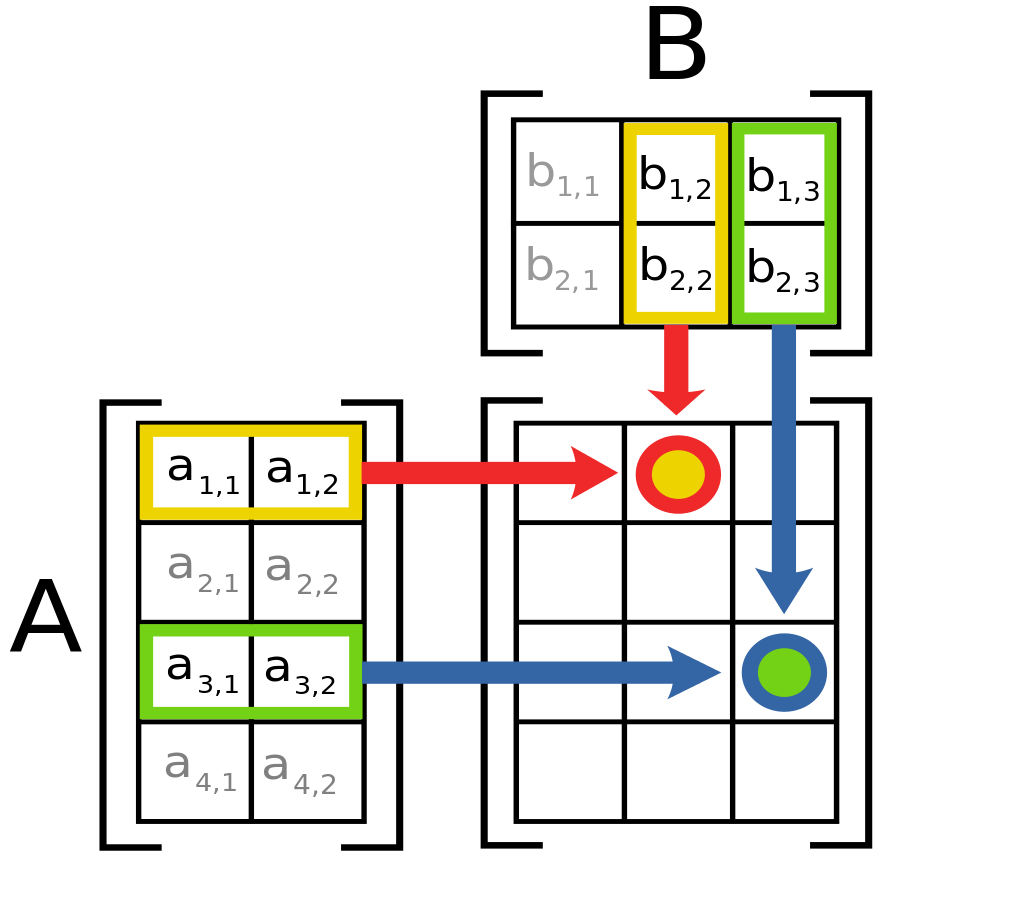
\includegraphics[width=.5\linewidth]{figures/Matrix_multiplication_diagram_2.png}
        %Source: \url{https://en.wikipedia.org/wiki/Matrix_multiplication#/media/File:Matrix_multiplication_diagram_2.svg}
      }
    \end{frame}

    \begin{frame}{The identity matrix}
      \begin{align}
        \mathbf{I} = \begin{pmatrix}
          1 & & & \\
            &1& & \\
            & & \ddots &\\
            & & &1\\
        \end{pmatrix}
      \end{align}
      \note{Demonstrate multiplication with the inverse by hand.
      \begin{align}
        \begin{pmatrix}
          -1 & 0 & 0 \\
           1 &-1 & 1 \\
           1 & 0 &-1
          \end{pmatrix}
        \begin{pmatrix}
          -1  &-0 &-0 \\
          -2  &-1 &-1 \\
          -1  &-0 &-1
        \end{pmatrix}
        =
        \begin{pmatrix}
           1  & 0 & 0 \\
           0  & 1 & 0 \\
           0  & 0 & 1
        \end{pmatrix}
      \end{align}
    }
    \end{frame}

    \begin{frame}{Matrix inverse}
      The inverse Matrix $\mathbf{A}^{-1}$ undoes the effects of $\mathbf{A}$, or in mathematical notation,
      \begin{align}
        \mathbf{A}\mathbf{A}^{-1} = \mathbf{I}.
      \end{align}
      The process of computing the inverse is called Gaussian elimination.
      \note{
        Example on the board:
        \begin{align}
          \mathbf{A} &= 
          \begin{pmatrix}
            2 & 0 \\
            1 & 3
          \end{pmatrix}
          \rightsquigarrow 
          \begin{pmatrix}[c c | c c]
            2 & 0 & 1 & 0 \\
            1 & 3 & 0 & 1\\ 
          \end{pmatrix}
          \rightsquigarrow
          \begin{pmatrix}[c c | c c]
            1 & 0 & \frac{1}{2} & 0 \\
            1 & 3 & 0 & 1\\ 
          \end{pmatrix} \\
          &\rightsquigarrow
          \begin{pmatrix}[c c | c c]
            1 & 0 & \frac{1}{2} & 0 \\
            0 & 3 & -\frac{1}{2} & 1\\ 
          \end{pmatrix}
          \rightsquigarrow
          \begin{pmatrix}[c c | c c]
            1 & 0 & \frac{1}{2} & 0 \\
            0 & 1 & -\frac{1}{6} & \frac{1}{3}\\ 
          \end{pmatrix}
      \end{align}
      Test the result:
      \begin{align}
          \begin{pmatrix}
            2 & 0 \\
            1 & 3 \\
          \end{pmatrix}
        \begin{pmatrix}
          \frac{1}{2} & 0 \\
          -\frac{1}{6} & \frac{1}{3}\\ 
        \end{pmatrix}
      = 
        \begin{pmatrix}
          2 \cdot \frac{1}{2} + 0 \cdot -\frac{1}{6} & 2 \cdot 0 + 0 \cdot \frac{1}{3}  \\
          1 \cdot \frac{1}{2} + 3 \cdot -\frac{1}{6} & 0 \cdot 0 + 3 \cdot \frac{1}{3} 
        \end{pmatrix}
      =
      \begin{pmatrix}
        1 & 0 \\
        0 & 1 \\ 
      \end{pmatrix}
      \end{align}
      }
    \end{frame}


    \begin{frame}{The Transpose}
      The transpose operation flips matrices along the diagonal, for example, in $\mathbb{R}^2$,
      \begin{align}
        \begin{pmatrix}
          a & b \\
          c & d \\
        \end{pmatrix}^T
        =
        \begin{pmatrix}
          a & c \\
          b & d \\
        \end{pmatrix}
      \end{align}
    \end{frame}

    \begin{frame}{Motivation of the determinant}
      \begin{itemize}
        \item The determinant contains lots of information about a matrix in a single number.
        \item When a Matrix has a zero determinant, its inverse does not exist.
        \item We require determinants to find eigenvalues by hand.
      \end{itemize}
    \end{frame}

    \begin{frame}{Computing determinants in two or three dimensions}
      The two-dimensional case:
      \begin{align}
        \begin{vmatrix}
          a_{11} & a_{12} \\
          a_{21} & a_{22} \\
        \end{vmatrix}
        = a_{11} \cdot a_{22} - a_{12} \cdot a_{21} \\
      \end{align}
      Computing the determinant of a three-dimensional matrix.
      \begin{align}
        \begin{vmatrix}
          a_{11} & a_{12} & a_{13}  \\
          a_{21} & a_{22} & a_{23}  \\
          a_{31} & a_{32} & a_{33}
        \end{vmatrix}
        = a_{11} \cdot
         \begin{vmatrix}
          a_{22} & a_{23}   \\
          a_{32} & a_{33}   \\
         \end{vmatrix}  
         -
         a_{21} \cdot
         \begin{vmatrix}
          a_{12} & a_{13}   \\
          a_{32} & a_{33}   \\
         \end{vmatrix}  
        +
         a_{31} \cdot
         \begin{vmatrix}
          a_{12} & a_{13}   \\
          a_{22} & a_{23}   \\
         \end{vmatrix}  
      \end{align}
      \note{Example computation on the board:
      \begin{align}
      \begin{vmatrix}
          -1 & 0 & 0 \\
           1 &-1 & 1 \\
           1 & 0 &-1
      \end{vmatrix}
       &= -1 \cdot
       \begin{vmatrix}
        -1 & 1  \\
         0 & -1 \\
       \end{vmatrix}  
       -
       1 \cdot
       \begin{vmatrix}
        0 & 0  \\
        0 & -1 \\
       \end{vmatrix}  
      +
       1 \cdot
       \begin{vmatrix}
        0 & 0  \\
        -1 & 1  \\
       \end{vmatrix}  \\
       &= (-1) \cdot ((-1) \cdot (-1) - 0 \cdot 1)) - \\
       &\;\;\;\;\;  (0 \cdot (-1) - 0 \cdot 0) + 0 \cdot 1 -(-1) \cdot 0 \\
       &= -1
      \end{align}

    }
    \end{frame}

    \begin{frame}{Determinants in n-dimensions}
      \begin{align*}
      \begin{vmatrix}
        a_{11} & a_{21} & \dots & a_{1n} \\
        a_{21} & a_{22} & \dots & a_{2n} \\
        \vdots & \vdots &       & \vdots \\
        a_{m1} & a_{m2} & \dots & a_{mn}
      \end{vmatrix}
    = a_{11} \begin{vmatrix}
      a_{22} & \dots & a_{2n} \\
      \vdots &        & \vdots \\
      a_{m2} & \dots & a_{mn}
    \end{vmatrix}
    + a_{21} 
    \begin{vmatrix}
      a_{21} & \dots & a_{2n} \\
      \vdots &        & \vdots \\
      a_{m2} & \dots & a_{mn}
    \end{vmatrix}
    \\
    \dots 
     a_{m1}
    \begin{vmatrix} 
      a_{11} & \dots & a_{1n} \\
      a_{21} & \dots & a_{2n} \\
      \vdots &        & \vdots \\
    \end{vmatrix}
    \end{align*}
    \note{Draw the sign pattern on the board:
    \begin{align}
      \begin{vmatrix}
        + & - & + & \dots \\
        - & + & - &  \dots \\
        + & - & + &  \dots \\
        \vdots & \vdots & \vdots & \ddots \\
      \end{vmatrix}        
    \end{align}
    The determinant can be expanded along any column as long as the sign pattern is respected.
    }
    \end{frame}

    \begin{frame}{Summary}
      \begin{itemize}
        \item We saw some of the most important operations in linear algebra.
        \item Let's use these to do something useful next.
      \end{itemize}
    \end{frame}

  \section{Linear curve fitting}
    \begin{frame}{What is the best line connecting measurements?}
      \begin{figure}
      \centering
      \includestandalone{./figures/noisy_line}
      \end{figure}
    \end{frame}

    \begin{frame}{Problem Formulation}
      A line has the form $dx + c$, with $c,x,d \in \mathbb{R}$. In matrix language, we could ask for every point to be on the line,
      \begin{align}
        \begin{pmatrix}
          1 & x_1 \\ 
          1 & x_2 \\
          1 & x_3 \\
          \vdots  & \vdots \\ 
          1 & x_n \\
        \end{pmatrix}
        \begin{pmatrix}
          c \\ d \\
        \end{pmatrix}
        = 
        \begin{pmatrix}
          p_1 \\
          p_2 \\
          \vdots \\ 
          p_n  
        \end{pmatrix}.
      \end{align}
      We can treat polynomials as vectors, too! The coordinates populate the matrix rows in $\mathbf{A} \in \mathbb{R}^{n_p \times 2}$, and the coefficients
      appear in $\mathbf{x} \in \mathbb{R}^{2}$, with the points we would like to model in $\mathbf{b} \in \mathbb{R}^{n_p}$.
      The problem now appears in matrix form and can be solved using linear algebra!
    \end{frame}

    \begin{frame}{The Pseudoinverse \cite{strang2009introduction,deisenroth2020mathematics}}
      The inverse exists for square or $n$ by $n$ matrices.
      Nonsquare $\mathbf{A}$ such as the one we just saw, require the pseudoinverse,
        \begin{align}
          \mathbf{A}^{\dagger} = (\mathbf{A}^T\mathbf{A})^{-1}\mathbf{A}^T .
        \end{align}
      Sometimes solving $\mathbf{A}\mathbf{x} + \mathbf{b} = 0$ is impossible,
      the pseudoinverse considers,
        \begin{align}
          \min_x \dfrac{1}{2}|\mathbf{A}\mathbf{x} - \mathbf{b}|^2 \\
        \end{align}
      instead. $\mathbf{A}^{\dagger} \mathbf{b} = \mathbf{x}$ yields the solution.

    \note{
      Sometimes solving $\mathbf{A}\mathbf{x} + \mathbf{b} = 0$ is implossible.
      One the board, derive:
      \begin{align}
        \min_x \dfrac{1}{2}|\mathbf{A}\mathbf{x} - \mathbf{b}|^2 \\
      \end{align}
      At the optimum we expect,
      \begin{align}
        0 &= \nabla_x \dfrac{1}{2}|\mathbf{A}\mathbf{x} - \mathbf{b}|^2 \\
          &= \nabla_x \dfrac{1}{2}(\mathbf{A}\mathbf{x} - \mathbf{b})^T(\mathbf{A}\mathbf{x} - \mathbf{b}) \\
          &= (\mathbf{A}\mathbf{x} - \mathbf{b})\mathbf{A}^T \\
          &= \mathbf{A}^T\mathbf{A}\mathbf{x} - \mathbf{A}^T\mathbf{b} \\
          \mathbf{A}^T\mathbf{b} &= \mathbf{A}^T\mathbf{A}\mathbf{x} \\
          (\mathbf{A}^T\mathbf{A})^{-1}\mathbf{A}^T\mathbf{b} &= \mathbf{x}  
      \end{align}
    }
    \end{frame}

    \begin{frame}{Linear regression}
      \begin{figure}
        \includestandalone{./figures/regression}
      \end{figure}
    \end{frame}

    \begin{frame}{What about harder problems?}
      \begin{figure}
        \includestandalone{./figures/signal_complex}
      \end{figure}
    \end{frame}

    \begin{frame}{Fitting higher order polynomials}
      \begin{align}
        \underbrace{
        \begin{pmatrix}
          1       & x_1^1    & x_1^2  & \dots & x_1^m  \\ 
          1       & x_2^1    & x_2^2  & \dots & x_2^m  \\
          1       & x_3^1    & x_3^2  & \dots & x_3^m  \\
          \vdots  & \vdots    & \vdots  & \ddots & \vdots \\ 
          1       & x_n^1    & x_n^2  & \dots & x_n^m  \\
        \end{pmatrix}
        }_{\mathbf{A}}
        \underbrace{
        \begin{pmatrix}
          c_1 \\ c_2 \\ \vdots \\ c_m  
        \end{pmatrix}
        }_{\mathbf{x}}
        =
        \underbrace{
        \begin{pmatrix}
          p_1 \\
          p_2 \\
          \vdots \\ 
          p_n  
        \end{pmatrix}
        }_{\mathbf{b}}
        .
      \end{align}
      As we saw for the linear regression $\mathbf{A}^{\dagger}\mathbf{b} = \mathbf{x}$
      gives us the coefficients.
    \end{frame}

    \begin{frame}{Overfitting}
      The figure below depicts the solution for a polynomial of 7th degree, that is $m=7$.
      \begin{figure}
        \centering
        \includestandalone[scale=.9]{./figures/overfitting}
      \end{figure}
    \end{frame}

    \begin{frame}{Summary}
      \begin{itemize}
        \item We saw how linear algebra lets us fit polynomials to curves. 
        \item For the 7th degree polynomial the noise took over! What now?
      \end{itemize}
    \end{frame}

  \section{Regularization}

  \begin{frame}{Motivation}
    \begin{itemize}
      \item Is there a way to fix the previous example?
      \item To do so we start from a rather peculiar observation.
    \end{itemize}
  \end{frame}

  \begin{frame}{Eigenvalues and Eigen-Vectors}
    Multiply matrix $\mathbf{A}$ with vectors $\mathbf{x_1}$ and $\mathbf{x_2}$,
    \begin{align}
      \mathbf{A} = \begin{pmatrix}
        1 & 4 \\
        0 & 2 
      \end{pmatrix},
      \mathbf{x_1} = \begin{pmatrix}
        1 \\ 0
      \end{pmatrix},
        \mathbf{x_2} = \begin{pmatrix}
          4 \\
          1
     \end{pmatrix},
    \end{align}
    we observe
    \begin{align}
      \mathbf{A}\mathbf{x_1} = \begin{pmatrix}
        1 \\ 0
      \end{pmatrix},
      \mathbf{A}\mathbf{x_2} = \begin{pmatrix}
        8 \\ 2
      \end{pmatrix}
    \end{align}
    Vector $\mathbf{x_1}$ has not changed! Vector $\mathbf{x_2}$ was multiplied by two.
    In other words,
    \begin{align}
      \mathbf{A}\mathbf{x_1} = 1 \mathbf{x_1}, \mathbf{A}\mathbf{x_2} = 2 \mathbf{x_2} 
    \end{align}
  \end{frame}
  \begin{frame}{Eigenvalues and Eigenvectors}
    Eigenvectors turn multiplication with a matrix into multiplication with a number,
    \begin{align}
      \mathbf{A}\mathbf{x} = \lambda \mathbf{x} .
    \end{align}
    Subtracting $\lambda \mathbf{x}$ leads to,
    \begin{align}
      (\mathbf{A}\mathbf{x} - \lambda \mathbf{I}) \mathbf{x} = 0 \\
    \end{align}
    The interesting solutions are those were $\mathbf{x} \neq 0$, which means
    \begin{align}
      \det(\mathbf{A} - \lambda \mathbf{I}) = 0 
    \end{align}

  \note{On the board, compute the eigenvalues and vectors for the initial example.
  \begin{align}
  \mathbf{A}
  = \begin{pmatrix}
    1 & 4 \\
    0 & 2 
  \end{pmatrix}
  \rightarrow 
  \begin{vmatrix}
    1- \lambda & 4 \\
    0 & 2 - \lambda
  \end{vmatrix}
  = (1-\lambda)*(2-\lambda) - 0*4
   = 0 \\
  \rightarrow \lambda_1 = 1, \lambda_2 = 2 . \\
  \begin{pmatrix}
    1 - 1 & 4 \\
    0 & 2 - 1 
  \end{pmatrix}
  =
  \begin{pmatrix}
    0 & 4 \\
    0 & 1 
  \end{pmatrix}
  \mathbf{x}_1 = 0
  \rightarrow \mathbf{x}_1 = \begin{pmatrix}
    p \\ 0 
  \end{pmatrix} \text{ for } p \in \mathbb{R} \\
  \begin{pmatrix}
    1 - 2 & 4 \\
    0 & 2 - 2 
  \end{pmatrix}
  =
  \begin{pmatrix}
    -1 & 4 \\
    0 & 0 
  \end{pmatrix}
  \mathbf{x}_1 = 0
  \rightarrow \mathbf{x}_2 = \begin{pmatrix}
    q \\ \frac{1}{4}q 
  \end{pmatrix} \text{ for } q \in \mathbb{R}
  \end{align}
  \textit{Determinant not useful numerically, software packages use QR-Method.} 
    }
  \end{frame}


  \begin{frame}{Eigenvalue-Decomposition \cite{strang2009introduction}}
  Eigenvalues let us look into the heart of a sqaure system-matrix $\mathbf{A} \in \mathbb{R}^{n,n}$.
    \begin{align}
      \mathbf{A} 
      = \mathbf{S}\begin{pmatrix}
        \lambda_1 & & & \\
        & \lambda_2 & & \\
        & & \ddots    & \\
        & & & \lambda_n \\     
      \end{pmatrix}
      \mathbf{S}^{-1}
      =\mathbf{S}\Lambda \mathbf{S}^{-1},
    \end{align}
    with $\mathbf{S} \in \mathbb{R}^{n,n}$ and $\Lambda \in \mathbb{C}^{n,n}$. 
  \end{frame}

  \begin{frame}{Singular-Value-Decomposition \cite{strang2009introduction}}
    What about a non-square matrix $\mathbf{A} \in \mathbb{R}^{n,m}$? Idea:
    \begin{align}
      \mathbf{A^T}\mathbf{A} = \mathbf{V}
      \begin{pmatrix}
      \sigma_1^2 & & \\
      & \ddots & & \\
      & & \sigma_n^2   
      \end{pmatrix}
      \mathbf{V}^{-1},
      \mathbf{A}\mathbf{A^T} = \mathbf{U}
      \begin{pmatrix}
      \sigma_1^2 & & \\
      & \ddots & & \\
      & & \sigma_n^2   
      \end{pmatrix}
      \mathbf{U}^{-1}.
    \end{align}
    Using the eigenvectors of the $\mathbf{A}^T\mathbf{A}$ and $\mathbf{A}\mathbf{A}^T$ we construct, 
    \begin{align}
      \mathbf{A} = \mathbf{U}\Sigma \mathbf{V}^T,
    \end{align}
    with $\mathbf{A} \in \mathbb{R}^{m,n}$, $\mathbf{U} \in \mathbb{R}^{m,m}$, $\Sigma \in \mathbb{R}^{m,n}$ and $\mathbf{V} \in \mathbb{R}^{n,n}$ .
  \end{frame}

  \begin{frame}{Singular values and matrix inversion \cite{golub1965calculating}}
    \begin{align}
      \mathbf{A}^{\dagger} = \mathbf{V} \Sigma^\dagger \mathbf{U}^T = \mathbf{V} \begin{pmatrix}
      \sigma_1^{-1} & & \\
      & \ddots &  \\
      & & \sigma_m^{-1} \\ \hline 
      & 0 & \\
      \end{pmatrix} \mathbf{U}^T
    \end{align}
  \end{frame}

  \begin{frame}{Regularization via Singular Value Filtering}
  Originally we had a problem computing $\mathbf{A}^{\dagger}\mathbf{b} = \mathbf{x}$.
  To solve it, we compute,
  \begin{align} \label{eq:reg}
      \mathbf{x}_{reg} = \sum_{i=1}^{n} f_i \frac{\mathbf{u}_i^T b}{\sigma_i}\mathbf{v_i}
  \end{align}
  The filter factors are computed using $f_i = \sigma_i^2 / (\sigma_i^2 + \epsilon)$.
  Singular values $\sigma_i < \epsilon$ are filtered.
  Expressing equation \ref{eq:reg} using matrix notation:
  \begin{align}
    \mathbf{x}_{reg}= \mathbf{V} \mathbf{F} \begin{pmatrix}
      \sigma_1^{-1} & & & \\
      &  \ddots & \\
      &  & \sigma_m^{-1} \\ \hline
      & 0 &
    \end{pmatrix}
    \mathbf{U}^T \mathbf{b}_{noise}
  \end{align}
  with $\mathbf{A} \in \mathbb{R}^{m,n}$, $\mathbf{U} \in \mathbb{R}^{m,m}$, $\mathbf{V} \in \mathbb{R}^{n,n}$, $\mathbf{F} \in \mathbb{R}^{m,m}$, $\Sigma^{\dagger} \in \mathbb{R}^{n,m}$
  and $\mathbf{b} \in \mathbb{R}^{n,1}$.
  \end{frame}

  \begin{frame}{Regularized solution}
    \begin{figure}
      \includestandalone{./figures/regularized}
    \end{figure}
  \end{frame}

  \begin{frame}{Conclusion}
    \begin{itemize}
      \item True scientists know what linear can do for them!
      %\footnote{Originally: "True Engineers know what linear can do for them." \url{https://onderwijsaanbod.kuleuven.be/syllabi/e/H0M82AE.htm#activetab=doelstellingen_idp41632}}
      \item Think about matrix shapes. If you are solving a problem, rule out all formulations where the shapes don't work.
      \item Regularization using the SVD is also known as Tikhonov regularization.
    \end{itemize}
  \end{frame}

  \begin{frame}{Literature}
    \printbibliography
  \end{frame}

\end{document}
